\documentclass[12pt]{article}

\usepackage{graphicx}

\begin{document}

\title{GrantSeer Documentation 1.0}
\author{Yang Song \\ yxs176@cse.psu.edu \\\\ Pennsylvania State University}
\date{}
\maketitle

\section{Introduction}
This document aims to guide you design reusable apps and loosely coupled system specifically based on new GrantSeer. GrantSeer originally developed by Dr. Puck Treeratpituk and written in Ruby on Rail. However, to improve the readability of the whole project and make it more maintainable, we decide to rewrite the system with Python and Django.

\subsubsection*{Who need to read this documentation}
\begin{enumerate}
	\item\ Anyone who wants to improve the current GrantSeer project.
	\item\ Anyone who wants to create new web apps that share the same database \texttt{csx\_exp}.
	\item\ Anyone who wants to know the very basic features about Django 1.6.
\end{enumerate}

\subsubsection*{Who shoud not read this documentation}
\begin{enumerate}
	\item\ Anyone who would like to know how to create a Django web app from zero.
	\item\ Anyone who works on a different database.
\end{enumerate}

The complete reference and tutorial of Django could be found at \\ https://docs.djangoproject.com/en/1.6/


\section{GrantSeer Architecture}
As we want to decouple the whole system, new GrantSeer is split into two services: \texttt{GrantSeerFrontendService} and \texttt{SeerBackendService}. In service design pattern, \texttt{Frontend Service} basically is responsible for interacting with users, generating request to \texttt{Backend Service} and rendering the data transferred from \texttt{Backend Service} for users. \texttt{Backend Service} is responsible for interacting with \texttt{MySQL} database, grouping and sorting those data and what not. In Django, \texttt{Backend Serivce} should be regarded as a data persistent layer of web app, even it could do more stuff.

\begin{figure}[!htb]
	\caption{GrantSeer Architecture}
	\label{grantseer_architecture}
	\centering
	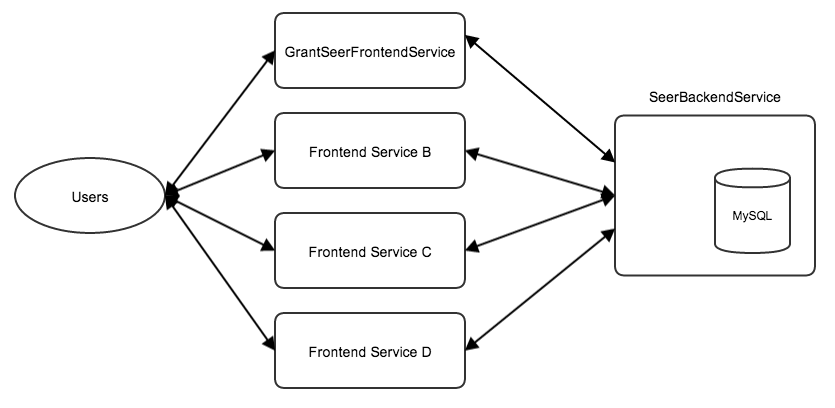
\includegraphics[width=\textwidth]{GrantSeerArchitecture.png}
\end{figure}

Figure \ref{grantseer_architecture} depicts architecture of GrantSeer. Currently only one frontend service exists. Developers are expected to add more frontend services that share the same database with \texttt{GrantSeer}. There are two reasons for this design.
\begin{enumerate}
	\item\ Distribute the workload. User requests only go to frontend services and different frontend services will handle different requests. \texttt{SeerBackendService} only handles requests that come from frontend services.
	\item\ Security. Only the ports that be able to reach frontend services are open. Malicious users are not be able to see \texttt{SeerBackendService}, so it's impossible to compromise backend service.
	\item\ Fail-safe. Even one or more frontend services are down, the rest of frontend services will be working normally.
\end{enumerate}

\section{Creating Frontend Service}
Your new frontend service should tightly-coupled with any other services in the current system, which means:
\begin{enumerate}
	\item\ Your frontend service should only send request to \texttt{SeerBackendService} and receive response from it.
	\item\ Your frontend service are NOT supposed to interact with other frontend services.
\end{enumerate}

















\end{document}
